% !TEX encoding = UTF-8 Unicode
\documentclass{report}

\title{Practical IT-Security: CSRF}
\author{Michael Müller}
\date{\today}
	
% big font for sections
\usepackage{sectsty}
\sectionfont{\LARGE}

\usepackage{graphicx}
\usepackage{wrapfig}
\usepackage{caption}
\usepackage{subcaption}
\usepackage{listings}
\usepackage{hyperref}

% \begin{comment} ... \end{comment{}
\usepackage{verbatim}

\setlength{\parskip}{0pt}

\makeatletter
\renewcommand{\paragraph}{
  \@startsection{paragraph}{4}
    {\z@}{1.25ex \@plus 1ex \@minus .2ex}{-1em}
      {\normalfont\normalsize\bfseries}
      }
      \makeatother


\begin{document}

\newpage

\maketitle

\newpage


%=================
\section{Introduction}

Cross-Site-Request-Forgery (\textsc{CSRF}) is an attack on web-applications
which will be further explained within the presentation.
This document is meant as a preparation document in order to get you ready to
understand the presentation and conduct the assignments.

\begin{comment}
\subsection{HTTP}
The HTTP protocol is the driving force behind the web.

\subsubsection{GET}
foo ar



\begin{lstlisting}[
	caption=Typical HTTP GET request
]
GET / HTTP/1.1
Host: google.com
\end{lstlisting}

\begin{lstlisting}[
	caption=Typical HTTP GET reply
]
200 OK 
\end{lstlisting}

\subsubsection{POST}
\end{comment}


%=================
\subsection{Web Developer Tool}

We aim to exploit several services in the assignments. Most of the exploits
will be written in HTML in conjuction with JavaScript. For this purpose it
comes handy if you are familiar with the developer tool of some browser.
Most modern browsers come with some kind of developer tools. Check the
corresponding manual or install a fitting plugin like FireBug (for Firefox). 
For Chromium the developer tools are accessible via ``\emph{Tools > Developer 
Tools}'' (or via pressing \texttt{F12}).
The main features of the developer tools, which will come handy for us, are: 

\paragraph{The JavaScript Console}
Enables us to view JavaScript errors in exploits.
\begin{figure}[h!]
	\centering
	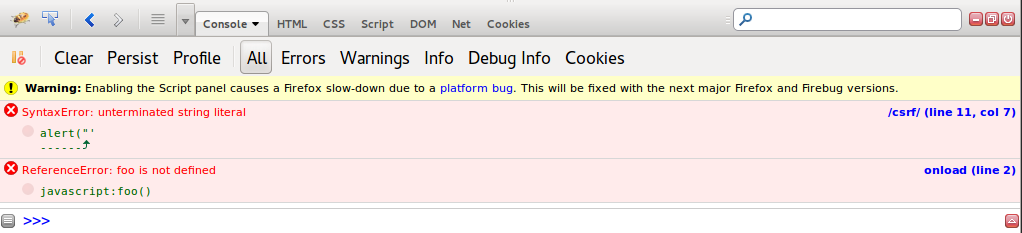
\includegraphics[width=1.0\textwidth]
		{./images/jsconsole.png}
	\caption{
		Beware: the Security level is set only temporarily as a
		Cookie!
	}
	\label{fig:jsconsole}
\end{figure}

\paragraph{The Network Capturer}
Enables us to analyze and debug the HTTP requests and replies which area
executed by the browser.
\begin{figure}[h!]
	\centering
	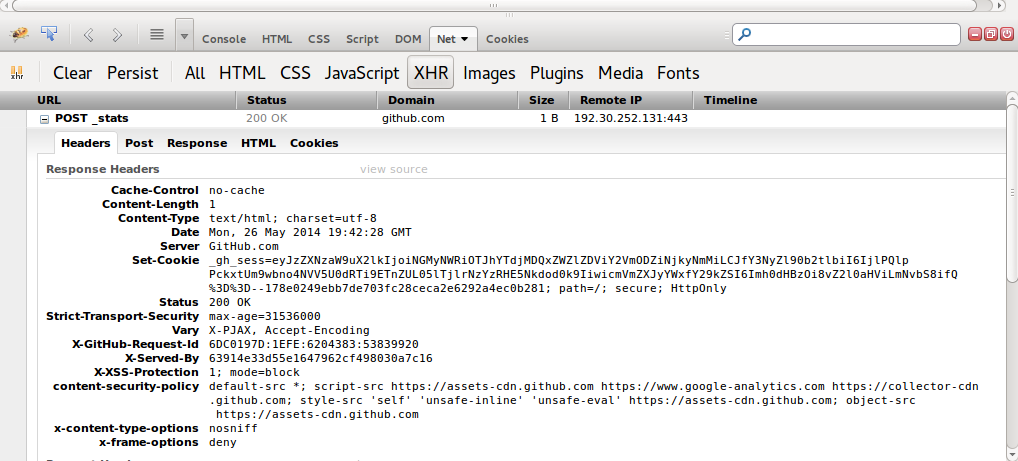
\includegraphics[width=1.0\textwidth]
		{./images/httpcapturer.png}
	\caption{
		Beware: the Security level is set only temporarily as a
		Cookie!
	}
	\label{fig:httpcapturer}
\end{figure}


%=================
\section{Assignments}

To carry out the assignments you need to bring your own laptop configured
to the run the services described in this section.

\subsection{Metasploitable}
We will continue to use the Metasploitable image, which has been provided 
in the warm-up phase of the course. If you no longer have it at hand you
should download it from the 
\href{https://moodle.uni-ulm.de/course/view.php?id=1312}{Moodle} platform
again. 

Use a software like for example VirtualBox, to get the image running
as a virtual machine (vm). Configure the vm in a way that you have
access to it over network (e.g. by configuring a Bridged Adapter within 
VirtualBox). If network access does not work out of the box you may
have to log into Metasploitable (User: \texttt{msfadmin}, Password:
\texttt{msfadmin}) and execute ``\texttt{\$ sudo dhclient eth0}'' in order
to obtain an IP address.

If everything worked you should be able to access the web server of the
vm from your host machine, e.g. if the vm runs on
192.168.1.103 via
\href{http://192.168.1.103/}{http://192.168.1.103/}.

\subsection{Damn Vulnerable Web App}
After you have completed the installation you should log into the
application to get a feeling for the interface.
Open up \href{http://192.168.1.103/dvwa}{http://192.168.1.103/dvwa}
and login with the credentials User: \texttt{admin}, Password: 
\textt{password}.
Open the navigation tab
\texttt{DVWA Security} and configure \texttt{Security Level: Low} (see
Figure \ref{fig:dvwa0}).

During the assignment we will work our way through the security levels 
\texttt{low} and \texttt{medium}. The level \texttt{high} is meant to show 
the state of the art best-practice solution. It is not meant to be cracked.\\

\textbf{Note:} The security level, which you configure is saved as a cookie 
value. The default value is \texttt{high}. This might lead to problems
while debugging: if you e.g. log into DVWA using Chromium and configure
\texttt{low} you should also run your exploit in Chromium and not 
in e.g. Firefox. Firefox would still be configured for the security level
\texttt{high}.

\begin{figure}[h!]
	\centering
	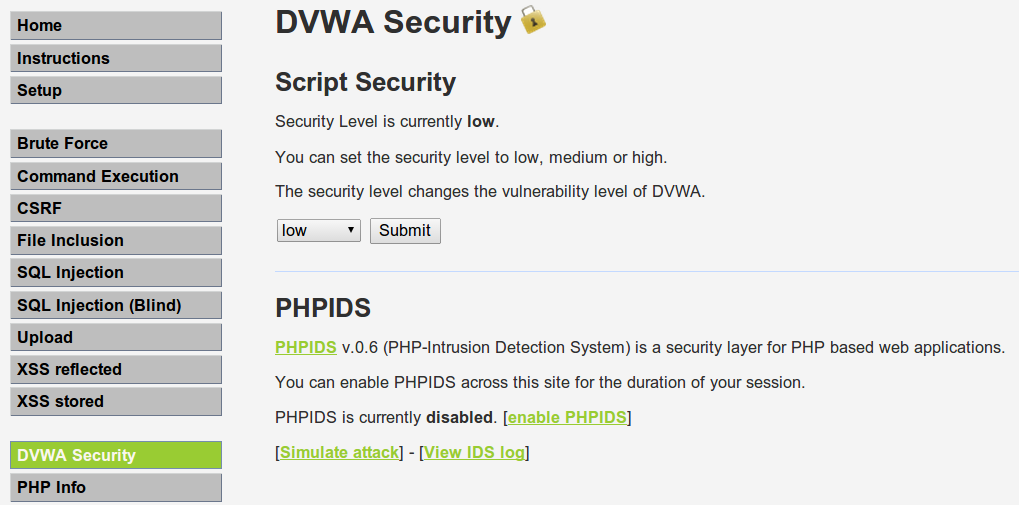
\includegraphics[width=0.8\textwidth]
		{./images/dvwa-security.png}
	\caption{
		Beware: the Security level is set only temporarily as a
		Cookie!
	}
	\label{fig:dvwa0}
\end{figure}

\section{Quick Checklist}

\paragraph{You should bring a basic understanding of}
\ \\
HTTP, HTML, the DOM, JavaScript.

\paragraph{You should bring}
\ \\
A laptop. Configured to run the Metasploitable image. Damn 
Vulnerable Web App should also be installed.

\paragraph{You should have played with}
\ \\
A Web Developer Tool.

\paragraph{You should be willing}
to enjoy learning something new and nibble on puzzles.

\center
\ \\
\texttt{-> happy hacking :] <-}

\end{document}
